% % arara: xelatex
% % arara: xelatex
% % arara: xelatex


% % options:
% % thesis=B bachelor's thesis
% % thesis=M master's thesis
% % czech thesis in Czech language
% % english thesis in English language
% % hidelinks remove colour boxes around hyperlinks

% \documentclass[thesis=B,english]{FITtemplates/FITthesis}[2019/12/23]

% %\usepackage[utf8]{inputenc} % LaTeX source encoded as UTF-8
% % \usepackage[latin2]{inputenc} % LaTeX source encoded as ISO-8859-2
% % \usepackage[cp1250]{inputenc} % LaTeX source encoded as Windows-1250

% % \usepackage{subfig} %subfigures
% % \usepackage{amsmath} %advanced maths
% % \usepackage{amssymb} %additional math symbols

% \usepackage{dirtree} %directory tree visualisation

% % % list of acronyms
% % \usepackage[acronym,nonumberlist,toc,numberedsection=autolabel]{glossaries}
% % \iflanguage{czech}{\renewcommand*{\acronymname}{Seznam pou{\v z}it{\' y}ch zkratek}}{}
% % \makeglossaries

% % % % % % % % % % % % % % % % % % % % % % % % % % % % % % % 
% % EDIT THIS
% % % % % % % % % % % % % % % % % % % % % % % % % % % % % % % 

% \department{Department of Applied Mathematics}
% \title{Autonomous car chasing}
% \authorGN{Pavel} %author's given name/names
% \authorFN{Jahoda} %author's surname
% \author{Pavel Jahoda} %author's name without academic degrees
% \authorWithDegrees{Pavel Jahoda} %author's name with academic degrees
% \supervisor{Ing. Jan Čech, Ph.D.}
% \acknowledgements{THANKS (remove entirely in case you do not with to thank anyone)}
% \abstractEN{Summarize the contents and contribution of your work in a few sentences in English language.}
% \abstractCS{V n{\v e}kolika v{\v e}t{\' a}ch shr{\v n}te obsah a p{\v r}{\' i}nos t{\' e}to pr{\' a}ce v {\v c}esk{\' e}m jazyce.}
% \placeForDeclarationOfAuthenticity{Prague}
% \keywordsCS{Replace with comma-separated list of keywords in Czech.}
% \keywordsEN{Replace with comma-separated list of keywords in English.}
% \declarationOfAuthenticityOption{1} %select as appropriate, according to the desired license (integer 1-6)
% % \website{http://site.example/thesis} %optional thesis URL


% \begin{document}

% % \newacronym{CVUT}{{\v C}VUT}{{\v C}esk{\' e} vysok{\' e} u{\v c}en{\' i} technick{\' e} v Praze}
% % \newacronym{FIT}{FIT}{Fakulta informa{\v c}n{\' i}ch technologi{\' i}}

% \setsecnumdepth{part}
% \chapter{Introduction}



% \setsecnumdepth{all}
% \chapter{State-of-the-art}

% \chapter{Analysis and design}

% Přidáme odstavec Text --- zejména ten odborný --- je nutné členit na odstavce. Každý odstavec by se měl týkat jednoho tématu, myšlenky\dots{} Odstavce od sebe musí být vizuálně oddělené. K tomu existuje několik vhodných stylů, které si popíšeme v jedné z následujících kapitol. Odstavce mohou být různě vysázené. V odborných textech je běžná sazba "do bloku". Při ní je nutné vhodně měnit mezislovní mezery. Jejich doporučená velikost je 0,25--0.33 čtverčíku.

% Požadavky jsou těchto typů:

% \chapter{Realisation}

% \setsecnumdepth{part}
% \chapter{Conclusion}


% \bibliographystyle{iso690}
% \bibliography{mybibliographyfile}

% \setsecnumdepth{all}
% \appendix

% \chapter{Acronyms}
% % \printglossaries
% \begin{description}
% 	\item[GUI] Graphical user interface
% 	\item[XML] Extensible markup language
% \end{description}


% \chapter{Contents of enclosed CD}

% %change appropriately

% \begin{figure}
% 	\dirtree{%
% 		.1 readme.txt\DTcomment{the file with CD contents description}.
% 		.1 exe\DTcomment{the directory with executables}.
% 		.1 src\DTcomment{the directory of source codes}.
% 		.2 wbdcm\DTcomment{implementation sources}.
% 		.2 thesis\DTcomment{the directory of \LaTeX{} source codes of the thesis}.
% 		.1 text\DTcomment{the thesis text directory}.
% 		.2 thesis.pdf\DTcomment{the thesis text in PDF format}.
% 		.2 thesis.ps\DTcomment{the thesis text in PS format}.
% 	}
% \end{figure}

% \end{document}




\documentclass{ctuthesis/ctuthesis}

\ctusetup{
	xdoctype = B,
	xfaculty = F8,
	mainlanguage = english,
	titlelanguage = english,
	title-english = {Autonomous Car Chasing},
	%title-czech = {Automaticke pronasledovani auta},
	department-english = {Department of Applied Mathematics},
	author = {Pavel Jahoda},
	supervisor = {Ing. Jan Čech, Ph.D.},
	supervisor-address = {Czech Technical University in Prague Faculty of Electrical Engineering  \\
	Center for Machine Perception},
	fieldofstudy-english = {Knowledge Engineering},
	keywords-czech = {samořídíci auto, RC auto, pronásledování, autonomní řízení, hluboké učení, CARLA, simulace},
	keywords-english = {self-driving car, RC car, chasing, autonomous driving, deep learning, CARLA, simulation},
	month = 5,
	year = 2020,
}

\ctuprocess

\begin{abstract-english}
We develop \ldots
\end{abstract-english}

\begin{abstract-czech}
Rozvíjíme \ldots
\end{abstract-czech}

% Acknowledgements / Podekovani
\begin{thanks}
I would like to express my deep gratitude to my supervisor Assistant Professor Ing. Jan Čech, Ph.D. for his patient guidance and willingness to devote his time to this work. I would also like to thank ToMi team (Michal Bahník, Dominik Filyo, Martin Vlašimský and others) who have assembled the 1:5 RC car platform used as the self-driving chasing car. Furthermore, I would like to thank doc. Ing. Martin Hromčík, Ph.D. for lending me his 1:10 RC car that was used as the chased car.\par

Finally, I would like to extend my thanks to my parents for their support throughout my education and to my girlfriend Vanda for her support and for helping me film promotional video of the autonomous car chase.
\end{thanks}

% Declaration / Prohlaseni
\begin{declaration}
		I hereby declare that the presented thesis is my own work and that I have cited all sources of information in accordance with the Guideline for adhering to ethical principles when elaborating an academic final thesis.
		
		I acknowledge that my thesis is subject to the rights and obligations stipulated by the Act No.\,121/2000~Coll., the Copyright Act, as amended. In accordance with Article~46~(6) of the Act, I hereby grant a nonexclusive authorization (license) to utilize this thesis, including any and all computer programs incorporated therein or attached thereto and all corresponding documentation (hereinafter collectively referred to as the ``Work''), to any and all persons that wish to utilize the Work. Such persons are entitled to use the Work in any way (including for-profit purposes) that does not detract from its value. This authorization is not limited in terms of time, location and quantity.
\end{declaration}



\begin{document}

\maketitle

\chapter{Introduction}
An autonomous car driving system capable of making fast and accurate decisions is important for making car transportation a safer activity. The reaction times of the system (especially in high speeds) have an impact on the human trust and acceptance of automated vehicles. The key aspects of driving autonomously include detecting other cars and interacting with them on the road. In this paper, we focus on testing a semi-autonomous system in these aspects by using a car chasing scenario. \par

A similar scenario -- car-following -- has been studied for more than half a century. Car-following models describe how drivers should follow each other in traffic stream. Oftentimes these theoretical models assume having precise data such as speed, distance and acceleration at every time-stamp \cite{car_following}. However, with the advancements of machine learning and computer vision more practical car-following models have been developed and tested. These models use sensors such as LIDAR and camera to estimate the distance between the two cars \cite{lidar_highway}. The estimated information is then used to maintain a safe distance between the two cars while following the trajectory of the front car. The car-following models have been however typically tested in scenarios that didn't involve high speeds and sudden significant speed changes. \par
 
 
On the other hand, a car chase -- vehicular hot pursuit of suspects by law enforcers -- typically involves high speeds and therefore fast reactions are necessary. In our scenario, a vehicle being pursued is driven by a person, while the vehicle that's chasing it is being controlled by an artificial intelligence-based system. The system architecture is similar to the DARPA Urban Challenge vehicles \cite{Bertha}\cite{darpa2}\cite{darpa_book} and consists of three parts: perception and localization, trajectory planning and a trajectory controller. \par


The thesis has the following structure. First, a theoretical background of the chasing algorithm is outlined. This includes related work and also a description of each part of the system. Then, a experiment section follows. The section includes testing in CARLA -- an open-source simulator for autonomous driving research. Additionally, it has a real-world evaluation of the system deployed in a radio-controlled car (RC car for short). The real-world evaluation consists of evaluation of a detector on a collected dataset and a practical chase in which the goal, similarly to the car-following model, is to maintain a determined distance between the two RC cars.

\chapter{Related work}

\chapter{Method}
\section{Overview}

\section{Computer vision}
\subsection{Convolutional Neural Network}
\subsection{Bounding Box Detector}
\subsection{Distance Estimation}
\subsection{Angle Estimation}

\section{Control And Planning}
\subsection{Pure Pursuit Algorithm}

\chapter{Experiments}

\section{Vehicle Detection}
\subsection{Dataset}
In order to train and evaluate 2D object detector capable of creating 2D bounding box around the chased RC car in a image, a dataset was needed. The collected dataset consists of \textbf{440} annotated images. All image annotations are in the PASCAL VOC data format introduced in the PASCAL Visual Object Classes Challenge \cite{pascal-voc}. Each image has it's annotation that contains pixel coordinates of the bounding box corners for each object in the image. In our dataset, only one object per image is present -- the chased RC car. The data were collected from multiple locations around Czechia and also under different lighting conditions. The majority of images were collected by the ZED Stereo camera attached to the chasing RC car. 


\subsection{Detection Results}

\section{Simulation}
\subsection{CARLA Environment}
\subsection{Experiment Setup}
\subsection{Results}

\section{Real-world Testing}
\subsection{RC Cars Description}
\subsubsection{Chasing RC car}
For deployment of our autonomous chasing algorithm a sub-scale vehicle platform called Toyota Mini (ToMi) was used %TODO cite. 
The platform is built around a large 1:5 scale RC car "Losi Desert Buggy XL-E 4WD". This electrically powered car has 0.9 x 0.5 meters length and width dimensions with reported maximal speed of up to 80km/h. At the core of the platform is a Raspberry Pi with a Navio-board that generates pulse width modulation signals for the throttle and steering to the servomotor. It is also equipped with a ZED stereo camera for taking color images, NVIDIA Jetson AGX Xavier graphics card for image processing and neural network interference. Finally, it is equipped with SSD to provide additional storage, GPS and IMU. \par
The whole simplified process flow is as follows. First, an image is taken by camera, which then goes to graphics card where it's analyzed by our algorithm. Then, based on the image analysis a steer and throttle values are updated. These values are transmitted from the graphics card to the Raspberry Pi which then sends signal to the servomotor that controls the vehicle.

\subsubsection{Chased RC car}
The RC car used as the chased vehicle is a 1:10 scale "Losi XXX-SCR RTR". This electrically powered car has 0.55 x 0.29 meters length and width dimensions with reported maximal speed of up to 55 km/h.

\begin{figure}[h!]
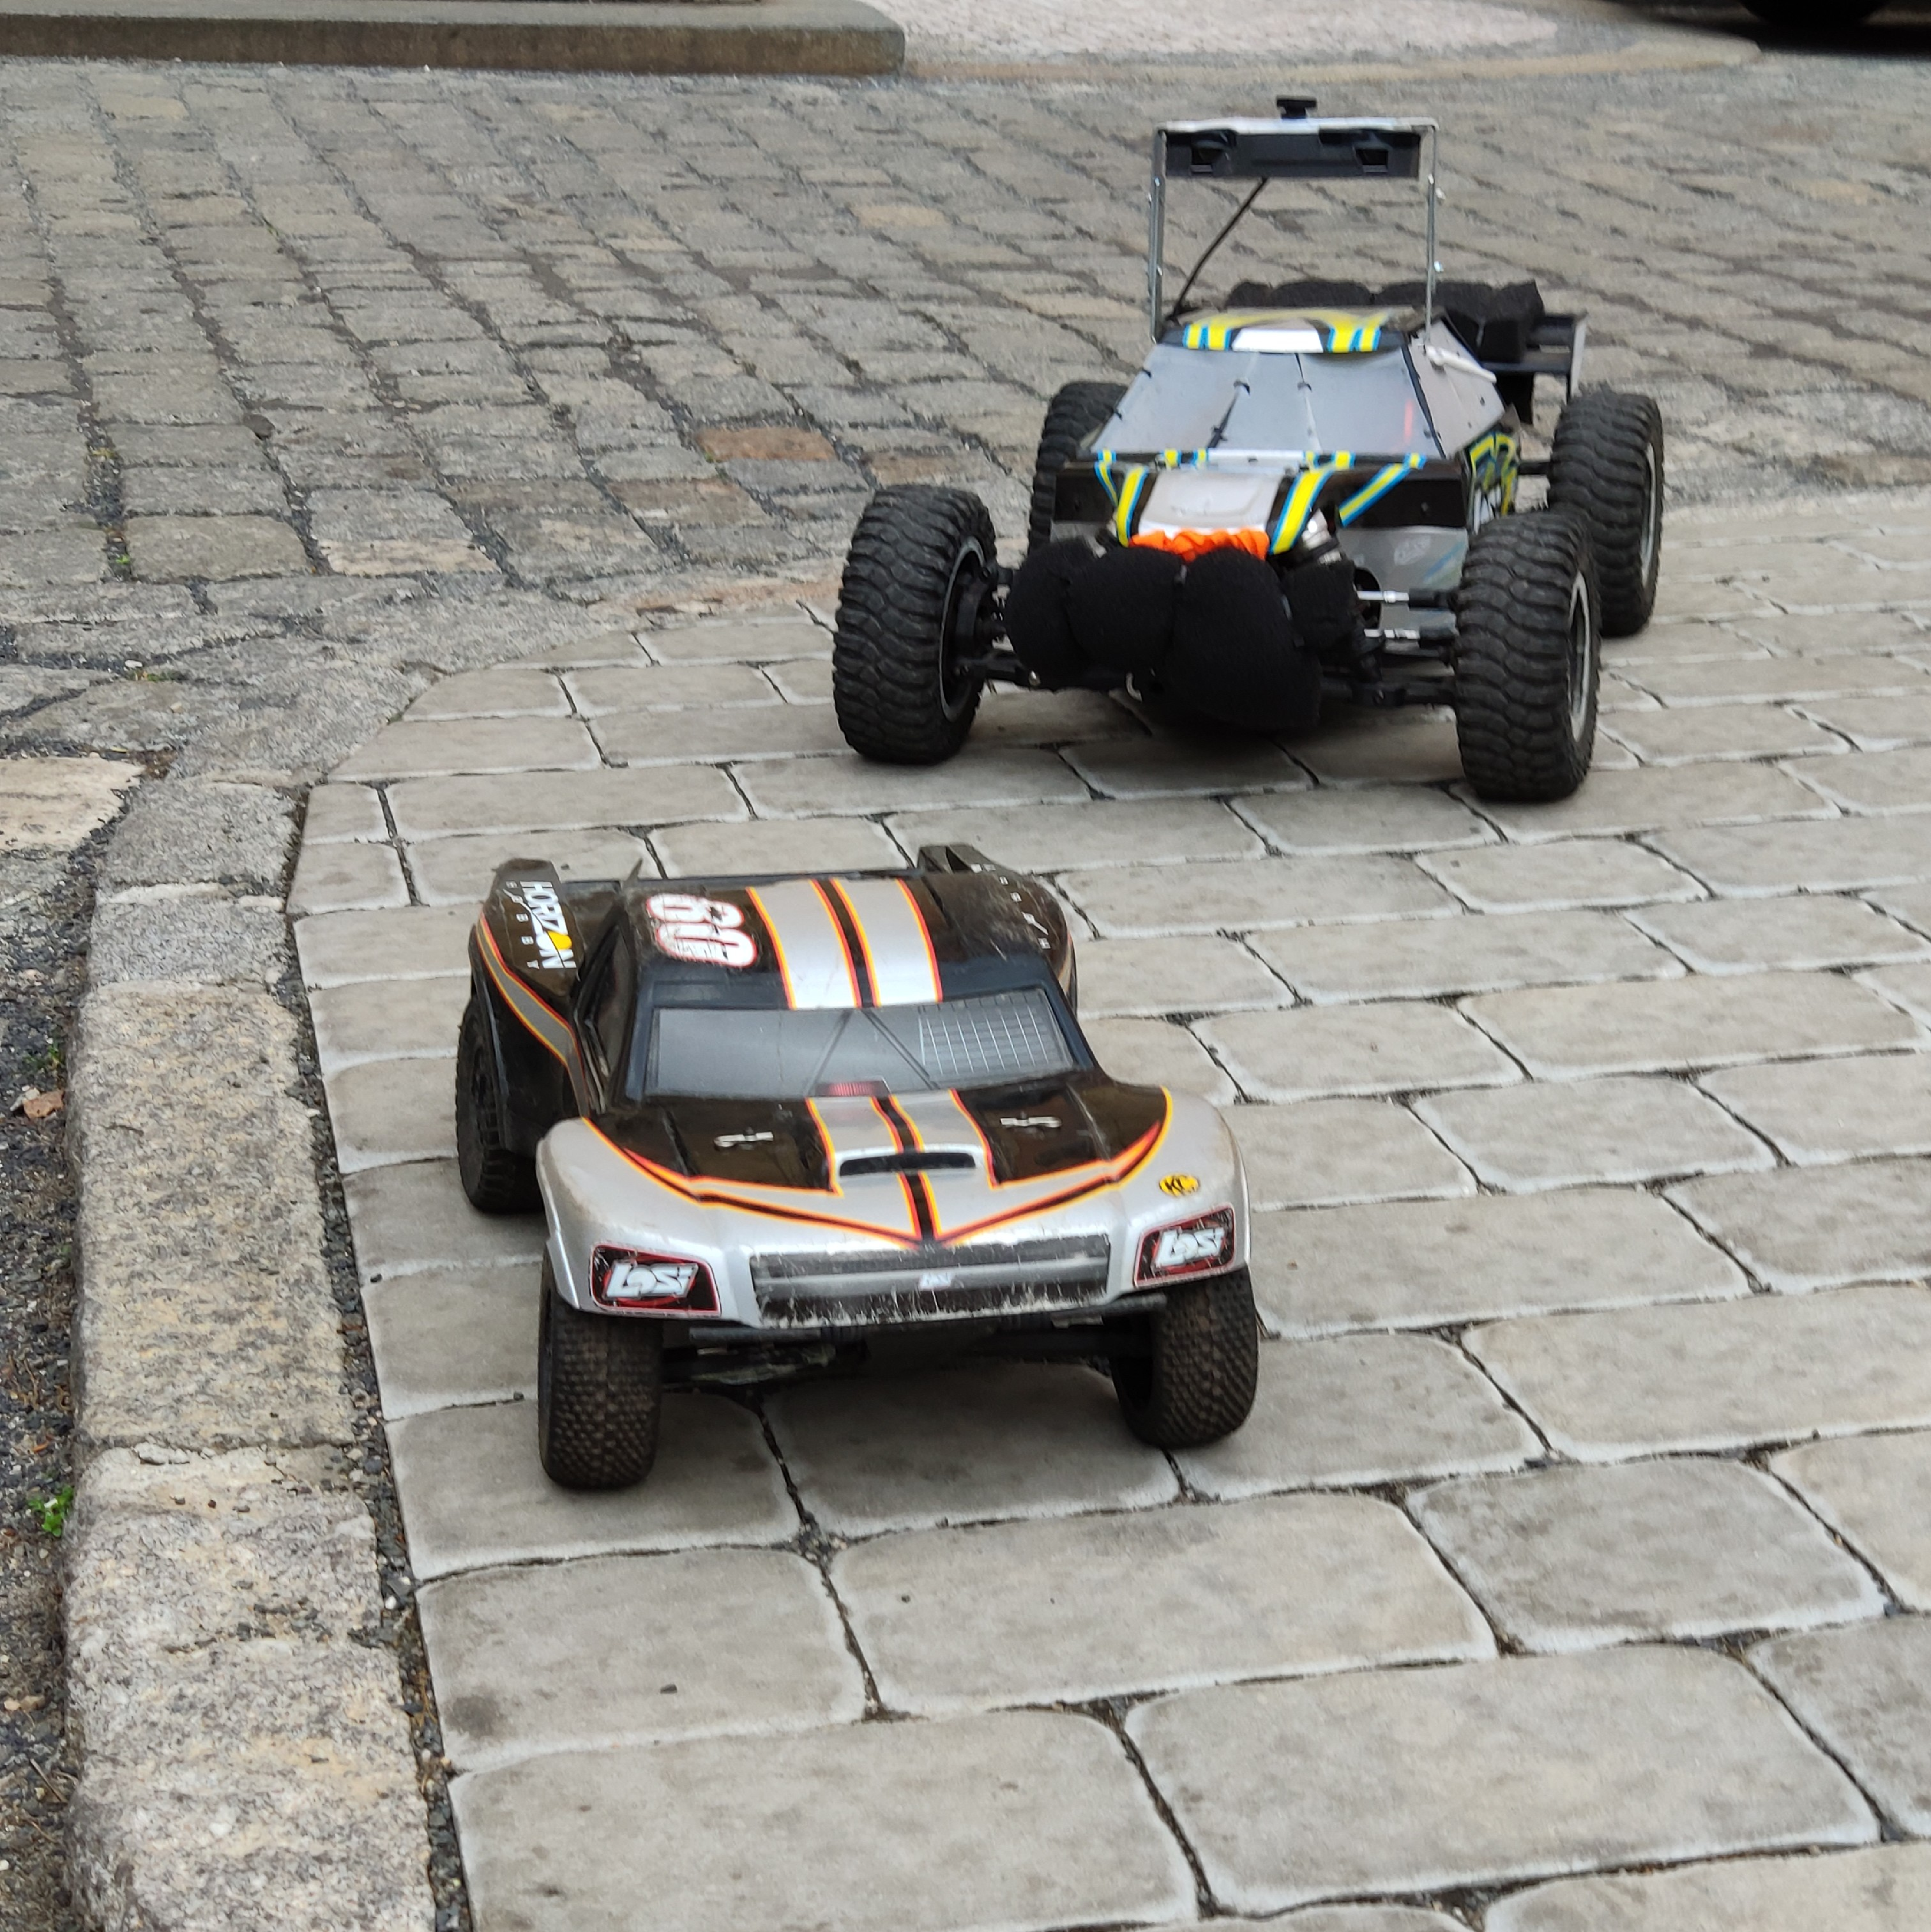
\includegraphics[width=0.5\textwidth]{images/rc_cars.pdf}
\caption{Both RC cars used for testing. The autonomous chasing car is in the back, while the manually driven car used as the pursued car is in the front}
\end{figure}


\subsection{Experiments}



\chapter{Conclusion}

\bibliography{citations}
\bibliographystyle{IEEEtran}

\end{document}

